
%%%%%%%%%%%%%%%%%%%%%%%%%%%%%%%%%%%%%%%%%%%%%%%%%%%%%%%%%%%%%%%%%%%%%%%%%%%%%
%%%%% CPP %%%%%%%%%%%%%%%%%%%%%%%%%%%%%%%%%%%%%%%%%%%%%%%%%%%%%%%%%%%%%%%%%%%
%%%%%%%%%%%%%%%%%%%%%%%%%%%%%%%%%%%%%%%%%%%%%%%%%%%%%%%%%%%%%%%%%%%%%%%%%%%%%
\fbckg{backgrounds/code2}
\begin{frame}
\pointedsl{C++}
\end{frame}

% based on http://ocw.mit.edu/courses/electrical-engineering-and-computer-science/6-096-introduction-to-c-january-iap-2011/index.htm

%%%%%%%%%%%%%%%%%%%%%%%%%%%%%%%%%%%%%%%%%%%%%%%%%%%%%%%%%%%%%%%%%%%%%%%%%%%%%
%%%%% History %%%%%%%%%%%%%%%%%%%%%%%%%%%%%%%%%%%%%%%%%%%%%%%%%%%%%%%%%%%%%%%
%%%%%%%%%%%%%%%%%%%%%%%%%%%%%%%%%%%%%%%%%%%%%%%%%%%%%%%%%%%%%%%%%%%%%%%%%%%%%
\begin{frame}
\frametitle{History}
\itemized{
	\item General-purpose programming language
	\item Created in 1979 by Bjarne Stroustrup
	\item Extension of C that includes
	\item Object-oriented programming, templating, polymorphism, operator overloading $\dots$
}
\end{frame}

%%%%%%%%%%%%%%%%%%%%%%%%%%%%%%%%%%%%%%%%%%%%%%%%%%%%%%%%%%%%%%%%%%%%%%%%%%%%%
%%%%% Compiling %%%%%%%%%%%%%%%%%%%%%%%%%%%%%%%%%%%%%%%%%%%%%%%%%%%%%%%%%%%%%
%%%%%%%%%%%%%%%%%%%%%%%%%%%%%%%%%%%%%%%%%%%%%%%%%%%%%%%%%%%%%%%%%%%%%%%%%%%%%
\fbckg{backgrounds/blank2}
\begin{frame}
\frametitle{Compiling}
\begin{center}
	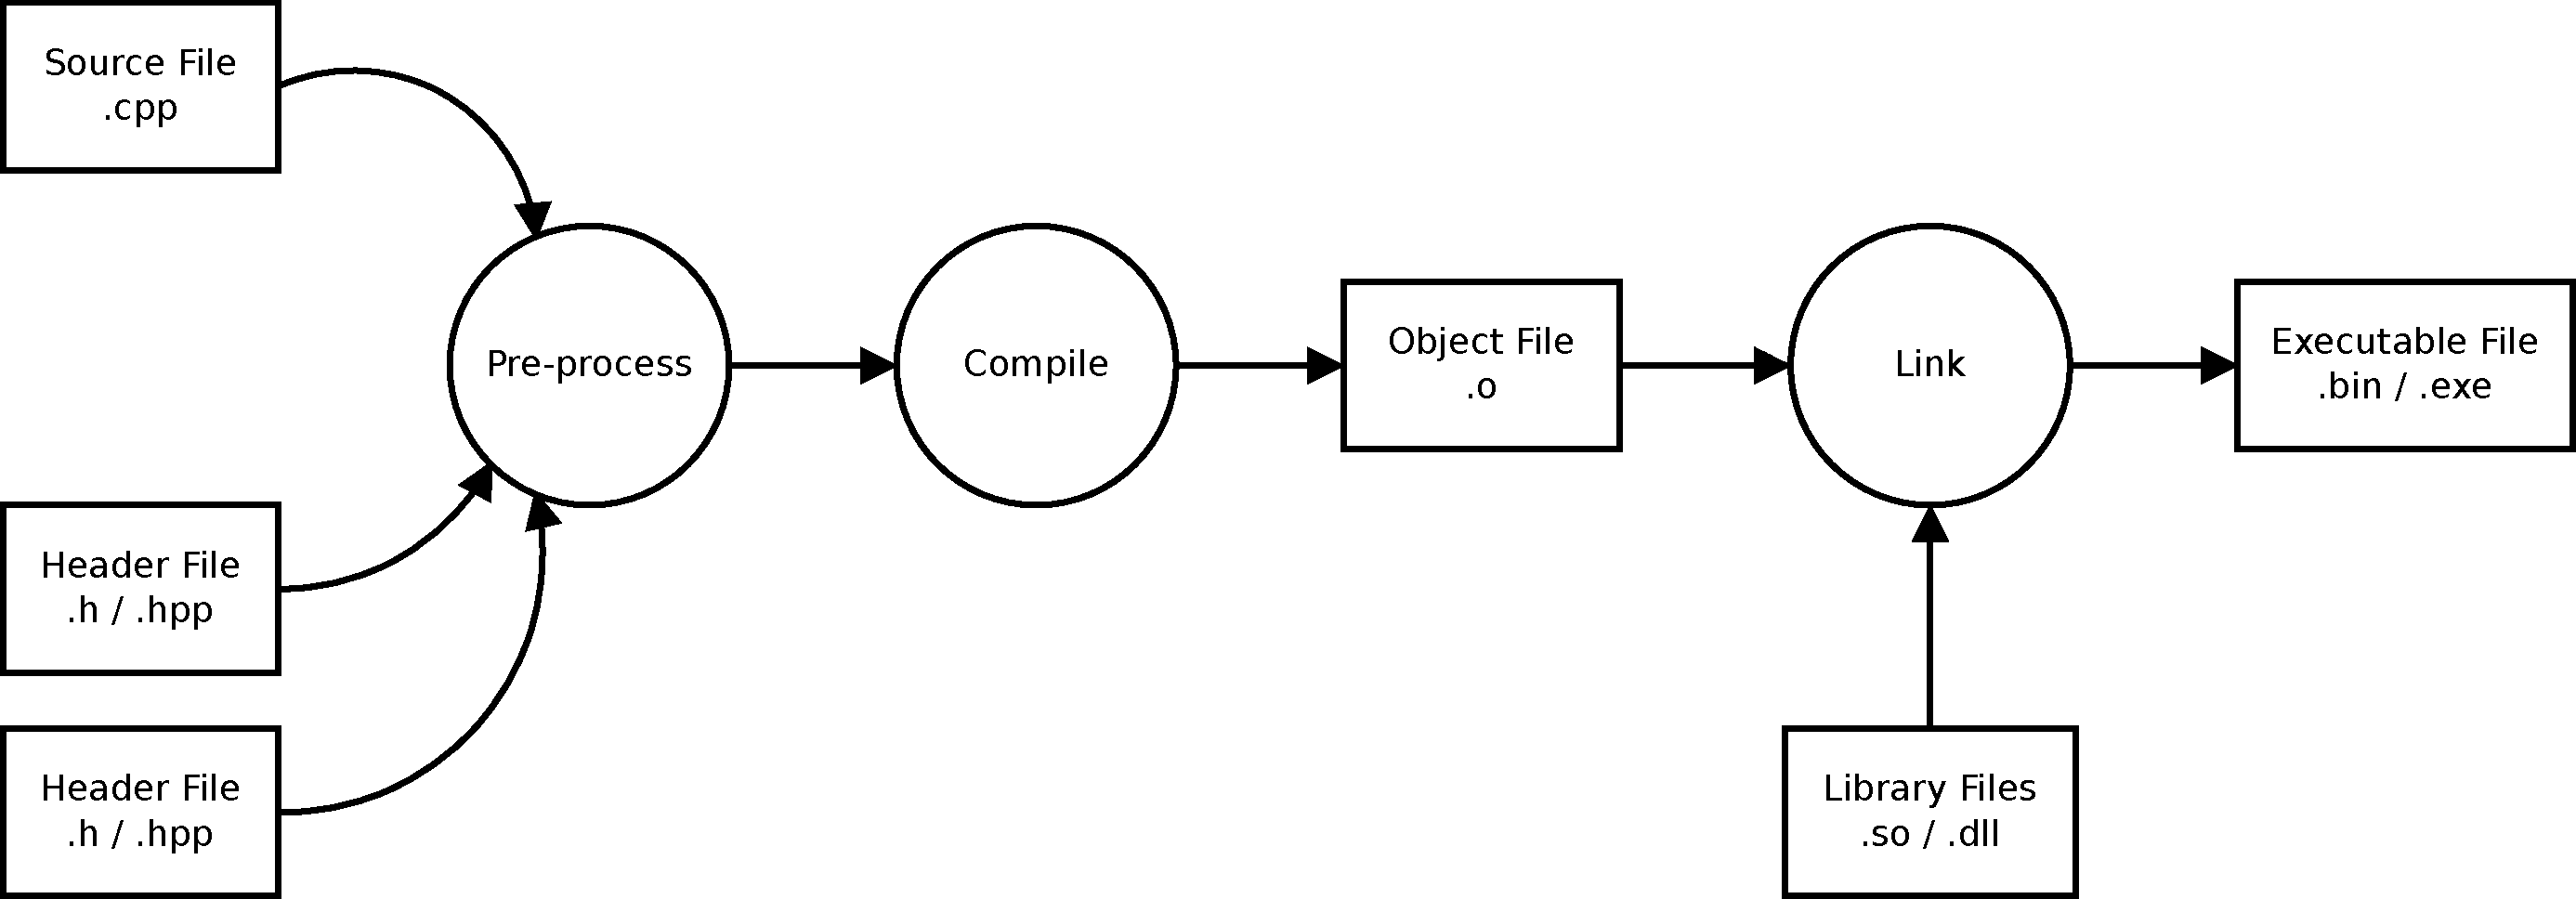
\includegraphics[width=0.97\textwidth]{figures/compiler}
	\end{center}
\misc{
	The \emph{compiler} translates source files (.cpp) into object files (.o).
	
	The \emph{linker} provides information to link object files (.o) together with libraries, producing an executable file (.exe).
}
\end{frame}

%%%%%%%%%%%%%%%%%%%%%%%%%%%%%%%%%%%%%%%%%%%%%%%%%%%%%%%%%%%%%%%%%%%%%%%%%%%%%
%%%%% Hello world %%%%%%%%%%%%%%%%%%%%%%%%%%%%%%%%%%%%%%%%%%%%%%%%%%%%%%%%%%%
%%%%%%%%%%%%%%%%%%%%%%%%%%%%%%%%%%%%%%%%%%%%%%%%%%%%%%%%%%%%%%%%%%%%%%%%%%%%%
\begin{frame}[fragile]
\frametitle{Hello World}
\begin{lstlisting}
#include<iostream>
// A comment
int main(int argc, char **argv){
    std::cout << "Hello world!\n";
    return 0;
}
\end{lstlisting}
\misc{
	Outputs "Hello world!" to the console and exits.
}
\end{frame}

%%%%%%%%%%%%%%%%%%%%%%%%%%%%%%%%%%%%%%%%%%%%%%%%%%%%%%%%%%%%%%%%%%%%%%%%%%%%%
%%%%% Pre-processor %%%%%%%%%%%%%%%%%%%%%%%%%%%%%%%%%%%%%%%%%%%%%%%%%%%%%%%%%
%%%%%%%%%%%%%%%%%%%%%%%%%%%%%%%%%%%%%%%%%%%%%%%%%%%%%%%%%%%%%%%%%%%%%%%%%%%%%
\begin{frame}[fragile]
\frametitle{Pre-processor instructions}
\begin{lstlisting}
#include<iostream>
\end{lstlisting}
\misc{
	Lines starting with a `\#' (pound) are instructions parsed by the \emph{pre-processor} such as
	\begin{itemize}
	\item \textbf{\#include} specifies a file to be included at this line.
	\item \textbf{\#if, \#ifdef, \#endif} conditionally uses a block of code.
	\item \textbf{\#define} creates an alias for an expression.
	\end{itemize}
}
\end{frame}

%%%%%%%%%%%%%%%%%%%%%%%%%%%%%%%%%%%%%%%%%%%%%%%%%%%%%%%%%%%%%%%%%%%%%%%%%%%%%
%%%%% Comments %%%%%%%%%%%%%%%%%%%%%%%%%%%%%%%%%%%%%%%%%%%%%%%%%%%%%%%%%%%%%%
%%%%%%%%%%%%%%%%%%%%%%%%%%%%%%%%%%%%%%%%%%%%%%%%%%%%%%%%%%%%%%%%%%%%%%%%%%%%%
\begin{frame}[fragile]
\frametitle{Comments}
\begin{lstlisting}[firstnumber=2]
// A comment (up to the end of the line)
\end{lstlisting}
\stext{or}
\begin{lstlisting}[firstnumber=2]
/* A comment 
possibly spanning
multiple lines */
\end{lstlisting}
\misc{
	are two types of comments, which the compiler ignores.
}
\end{frame}

%%%%%%%%%%%%%%%%%%%%%%%%%%%%%%%%%%%%%%%%%%%%%%%%%%%%%%%%%%%%%%%%%%%%%%%%%%%%%
%%%%% Main function %%%%%%%%%%%%%%%%%%%%%%%%%%%%%%%%%%%%%%%%%%%%%%%%%%%%%%%%%
%%%%%%%%%%%%%%%%%%%%%%%%%%%%%%%%%%%%%%%%%%%%%%%%%%%%%%%%%%%%%%%%%%%%%%%%%%%%%
\begin{frame}[fragile]
\frametitle{Main function}
\begin{lstlisting}[firstnumber=3]
int main(int argc, char **argv){
    ...
    return 0;
}
\end{lstlisting}
\misc{
	defines a function named \ctext{main} which
	\begin{itemize}
		\item takes two arguments \ctext{argc} and \ctext{argv},
		\item returns an integer value (\ctext{int} in front).
	\end{itemize}
	\phantom{.}
}
\end{frame}

\begin{frame}[fragile]
\frametitle{Main function (2)}
\begin{lstlisting}[firstnumber=3]
int main(int argc, char **argv){
    ...
    return 0;
}
\end{lstlisting}
\misc{
	The \ctext{main} function is called when the program starts, with
	\begin{itemize}
		\item \ctext{argc}, the number of arguments
		\item \ctext{argv}, the arguments (array of strings)
	\end{itemize}
	and returns an integer code ($0=$ success).
}
\end{frame}

%%%%%%%%%%%%%%%%%%%%%%%%%%%%%%%%%%%%%%%%%%%%%%%%%%%%%%%%%%%%%%%%%%%%%%%%%%%%%
%%%%% Output statement %%%%%%%%%%%%%%%%%%%%%%%%%%%%%%%%%%%%%%%%%%%%%%%%%%%%%%
%%%%%%%%%%%%%%%%%%%%%%%%%%%%%%%%%%%%%%%%%%%%%%%%%%%%%%%%%%%%%%%%%%%%%%%%%%%%%
\begin{frame}[fragile]
\frametitle{Output statement}
\begin{lstlisting}[firstnumber=4]
std::cout << "Hello world!\n";
\end{lstlisting}
\misc{
\begin{itemize}
	\item \ctext{std} is the standard \emph{namespace}.
	\item \ctext{cout} is a \emph{Stream} object.
	\item \ctext{<<} is the output operator of \emph{Stream}.
	\item \ctext{"Hello world"} is the string being output.
\end{itemize}
}
\end{frame}